\documentclass{../../text-style}
\texttitle{Введение, многопоточное программирование}

\begin{document}

\maketitle
\thispagestyle{empty}

\section{Введение}

\subsection{О чём курс}

Начнём с того, о чём вообще этот курс. В этом семестре считается, что вы уже освоили основы объектно-ориентированного программирования, поэтому в этом курсе будет рассказано, как же его применять. Вообще, цель этого курса --- познакомить вас с как можно большим количеством областей, с которыми должен быть знаком любой практикующий программист, чтобы после этого курса вы хотя бы слышали и имели небольшой опыт со всем, что обычно встречается программистам на практике. Это:

\begin{itemize}
    \item многопоточное программирование --- сейчас практически не бывает одноядерных процессоров, так что писать программы, имеющие всего один поток вычислений, становится всё более и более немодно; навыки многопоточного программирования считаются сейчас обязательными практически везде;
    \item сетевое программирование --- существуют кучи облачных сервисов и приложений, которые их используют, пользователи ожидают, что любая программа умеет загружать что-нибудь в какое-нибудь облачное хранилище, общаться с третьесторонними сервисами и т.д., без навыков сетевого программирования писать такие приложения очень сложно;
    \item веб-программирование --- можно сказать, что это подвид сетевого программирования, но вообще это отдельный мир, со своим стеком технологий, своими архитектурными подходами, своими даже языками программирования; к несчастью, большая часть создающихся нынче приложений --- именно веб-приложения, потому что они работают в браузере, не требуют установки и доступны на любой платформе (хоть на мобильнике) из любой точки мира;
    \item работа с базами данных --- без них в веб-программировании никуда, да и вообще, чтобы что-нибудь хранить, они необходимы;
    \item рефлексия --- вообще, она не очень нужна, но на ней построены многие из штук, про которые будет рассказываться, да и вообще, считается приличным уметь ей пользоваться;
\end{itemize}

Практически про каждый пункт из этого списка дальше (с третьего курса) будут спецкурсы, а времени у нас очень мало, поэтому может показаться, что про всё очень быстро и скомканно, но такова уж особенность этого курса. Относитесь к этому именно как к введению и к знакомству с каждой темой, потом, если понравится, можно будет более глубоко их изучить на старших курсах. Программа техпрога, к несчастью, устроена так, что почти все спецкурсы --- курсы по выбору, так что можно счастливо избежать всех этих знаний, но этот курс обязателен, так что необходимый минимум знаний всё-таки придётся получить.

\subsection{Отчётность}

С формальной точки зрения у нас, как в прошлом семестре, одна пара в неделю, в основном я буду что-то рассказывать, но будут и пары, где надо будет писать код прямо на паре. Например, про многопоточное программирование, про которое можно долго рассказывать, но при первой попытке что-нибудь сделать все всё равно простреливают себе ногу --- я сам это делал, даже в промышленных проектах. Или веб-приложения, где рассказывать ещё больше, но пока руками не попробуете, толку от этого мало. Будет две контрольные (одна где-то в середине семестра, одна в конце), доклады и, конечно, много домашки (задач будет меньше, чем в прошлом семестре, но они будут объёмнее).

\subsection{Шкала оценивания}

Каждая задача оценивается в несколько баллов (в зависимости от сложности задачи), есть максимальный балл за задачу и текущий балл за задачу. Максимальный балл можно терять, текущий балл увеличивать, и когда они встретятся, это и будет итоговая оценка за задачу. То же самое с контрольными --- единственное, что баллы за них нельзя улучшать, можно только переписать контрольную целиком. У нас всего две контрольные и три-четыре попытки, из попыток будут выбраны две лучшие оценки для расчёта итогового балла. В итоговой оценке баллы за домашки и контрольные учитываются следующим образом.

\begin{itemize}
    \item Баллы за домашки пересчитываются по формуле $MAX(0, (n/N – 0.6)) * 2.5 * 100$, где $n$ --- сумма текущих баллов за домашки, $N$ --- сумма баллов, которую в принципе возможно было получить за курс. То есть, надо получить хотя бы 60\% баллов, иначе за домашки у вас будет 0. Сколько вы сделаете от 60\% до 100\%, как раз и определяет, насколько высокую оценку вы получите.
    \item Баллы за контрольные считаются гораздо проще: $n/N * 100$, где $n$ --- это сумма ваших баллов за две лучшие попытки, $N$ --- максимум, что можно набрать за две попытки. Контрольных будет всего две, так что $N = 20$.
    \item Итоговый балл за курс получается как \textbf{минимум} из этих двух баллов. Так что если вы сделали всю домашку, но слили все контрольные --- скорее всего, домашку за вас сделал кто-то ещё и вас надо отчислить. Если вы сделали все контрольные идеально, но домашку не сделали, вы раздолбай и вас надо отчислить.
    \item Дальше всё очень просто --- если вы набрали больше 50\% баллов за курс, вам зачёт, если нет, то увы.
\end{itemize}

Чтобы получить зачёт, достаточно сдать 80\% домашек и половину контрольных (всего половину! Вы можете идеально написать контрольную 1, и на вторую вообще не ходить!). Кроме того, можно получить дополнительные баллы за активность в аудитории (у нас будет пара практических занятий, где успешное выполнение задания может принести немного баллов). Доклады стоят как целая домашка средней сложности по баллам, но достанутся не всем. Домашку можно не доделывать --- вы можете получить за неё, например, 7 баллов из 10, и не править всякие замечания типа нехватки комментариев.

У нас также будут дедлайны в 2-3 недели, за сдачу после дедлайна вы теряете по полбалла за каждую неделю пропуска. Кроме того, за каждую попытку сдачи после второй вы теряете тоже по полбалла. Один раз можно поправить бесплатно, потому что мы учимся, дальше вы штрафуетесь за то, что в реальной жизни очень сложно сказать <<ах да, не подумал, сейчас поправлю>>, если код уже на продакшене (или вообще улетел к Венере на космическом зонде). При этом задавать любые вопросы до сдачи никто не запрещает (кроме <<а сколько баллов я бы получил, если бы сдал сейчас>>, конечно). Кроме того, если задача на момент сдачи не выполняет все требования условия, вы сразу теряете баллы, пропорциональные объёму невыполненных требований (делить на два, так что если сдать пустой проект, максимальный балл сразу ополовинится). Это тоже отражение реальной жизни, вы не можете про какой-то пункт ТЗ при сдаче сказать <<ой, не заметил>>. И кроме того, за грубые ошибки в попытках сдачи после 2-й или неисправление замечаний я могу снимать до балла за каждую ошибку (например, выкладывание бинарников в git быстро обесценит решение). В любом случае, штрафы снижают баллы за задачу не более чем до половины её максимального балла, так что если вы весь семестр страдали фигнёй, вам на зимней сессии надо будет идеально сделать все задачи и решить ещё немного дополнительных. Дополнительные задачи выдаются только тем, кто не аттестован, и только после решения основных, так что ждать лёгкую задачу взамен сложной бесполезно.

\section{Многопоточность}

Многопоточное программирование ещё двадцать лет назад было чёрной магией, которую знали не очень многие практикующие программисты, и даже среди них умели писать нормальные многопоточные программы на практике далеко не все. Тридцать лет назад многопоточное программирование вообще упоминалось разве что в контексте высокопроизводительных вычислений на суперкомпьютерах. Кстати, так оно в основном до сих пор преподаётся на матмехе на спецкурсах, <<представьте себе, что у нас есть машина с бесконечным количеством процессоров>>. Однако в середине 2000-х произошла одна важная вещь --- закон Мура\footnote{закон Мура, URL: \url{https://ru.wikipedia.org/wiki/Закон\_Мура}, дата обращения: 31.08.2020} перестал работать. Миниатюризация процессоров и рост их тактовой частоты наткнулись уже на релятивистские ограничения, так что <<даром>> увеличивать производительность программ оказалось уже физически невозможно. 

Поэтому производители процессоров пошли <<вширь>>, создавая процессоры с несколькими ядрами, которые работают на не очень большой тактовой частоте, но могут заниматься несколькими задачами одновременно. Довольно типичный современный процессор, например, как у меня в ноутбуке, имеет на одном кристалле четыре независимых ядра (по сути, четыре отдельных процессора), способные исполнять восемь потоков одновременно, кеш-память, да ещё и графическую подсистему, играющую роль видеокарты. Проблема в том, что если запустить обычное однопоточное приложение (как мы всегда до этого писали) на таком процессоре, оно будет работать медленно, а загруженность процессора будет невысокой (на моей машине порядка 12\%, даже если приложение будет непрерывно делать вычислительно интенсивные операции), а добавление ещё ядер не даст ровным счётом ничего.

Помочь может распараллеливание программ. Хорошая вычислительно интенсивная программа должна использовать все или почти все ресурсы процессора для полезной работы, поэтому она принципиально должна быть многопоточной. Одноядерных процессоров в реальном мире практически не бывает (по крайней мере, общего назначения, во встроенных системах встречаются, но это отдельный мир), так что если вы дедовскими методами пишете всё в один поток, в современном мире это не очень.

Кроме того, многопоточность нужна и для адекватной реализации программ, использующих длительные операции ввода-вывода. Например, загрузка большого файла в память может быть не вычислительно сложной (на самом деле, этим процессор, как правило, вообще не занимается, это делает специальная микросхема DMA), но может занимать длительное время. То же касается сетевых операций. Тем более, если можно выполнять несколько таких операций одновременно (например, BitTorrent --- файл в torrent-протоколе качается из десятков источников одновременно). К тому же, при завершении операции программа должна продолжить работу с того места, где она остановилась. При этом (пожалуй, самое главное) во время операции программа должна реагировать на действия пользователя: если у неё есть GUI, он должен реагировать на клики, перерисовываться, даже показывать прогресс. Это тоже реализуется несколькими потоками.

Получается, что любая или практически любая современная программа так или иначе многопоточна. Почему же тогда мы не проходили многопоточность на первом курсе --- потому что есть тысяча способов сделать всё неправильно и даже не понять, что что-то не так. Многопоточные программы обладают тем удивительным свойством, что доказательство корректности их работы, как правило, алгоритмически неразрешимо, а сами ошибки могут проявляться очень редко, буквально раз в тысячу лет, так что тестированием их не найти. Связано это с тем, что переключение потоков принципиально недетерминированно --- вы не можете знать, когда операционная система приостановит один из ваших потоков и даст поработать другому (вашему или не вашему). Буквально после каждой инструкции в программе управление может быть передано куда-то ещё. И даже \textbf{посреди} инструкции, если речь идёт про языки высокого уровня, как C\#.

Более того, не всегда многопоточная программа работает быстрее однопоточной. На одноядерном процессоре многопоточная вычислительно интенсивная программа всегда будет работать медленнее такой же однопоточной, иногда заметно медленнее. Даже если всё хорошо, далеко не любой алгоритм можно распараллелить, и далеко не любое распараллеливание приведёт вас к успеху. 

Собственно, подробности про все эти тонкости мы подробно обсудим за ближайшие четыре пары и, самое важное, в домашках. Вас немного потом ждёт одна особо злая задача, про которую даже не предполагается, что вы её решите с первого раза (и количество бесплатных попыток для неё будет увеличено).

\subsection{Процессы и потоки}

Немного терминологического ликбеза:

\begin{itemize}
    \item \textbf{Процесс} --- это исполняющаяся программа. То есть загруженный операционной системой в память .exe-шник со всеми .dll-ками, от которых он зависит (или бинарник и .so-шки в Linux). Одной программе может соответствовать несколько процессов (никто не мешает вам запустить программу несколько раз), так что процесс можно понимать как экземпляр программы.
    \begin{itemize}
        \item Процесс имеет связанные с ним системные ресурсы --- это его память, открытые им файлы, открытые сетевые соединения и прочие подобные системные ресурсы. Кстати, современные операционные системы реализуют механизм \textit{виртуальной} памяти, так что процесс думает, что ему выделен просто непрерывный массив памяти от 0 до пары терабайт, даже несмотря на то, что оперативки в обычных компьютерах столько не бывает, и процесс в операционной системе не один. ОС делает так, чтобы процесс не видел чужую память и даже не подозревал о её существовании.
    \end{itemize}
    \item \textbf{Поток} --- это часть процесса, соответствующая потоку исполнения. До этого у нас были процессы, содержащие один поток, но, как вы догадались, в процессе потоков может быть много. Каждый поток имеет свой стек вызовов, своё состояние регистров процессора (при переключении потока ОС сохраняет текущее содержимое регистров и восстанавливает при переключении обратно). Это позволяет фактически в одной программе иметь сразу несколько независимых друг от друга текущих исполняемых инструкций (говоря образно и на примере Visual Studio, несколько <<жёлтых стрелочек>> в отладчике). При этом все потоки разделяют общую память процесса, так что могут легко общаться через общие переменные (на самом деле, это боль, но про это чуть потом). И разделяют общие системные ресурсы процесса, такие как открытые файлы. Кстати, стек вызовов у каждого потока свой, поэтому \textbf{все локальные переменные у каждого потока свои}. А вот всё, что на куче, у всех потоков общее. А поскольку любой ссылочный тип в C\# выделяется на куче, то... ну, вы поняли.
\end{itemize}

\subsection{Виды параллельных программ}

Когда говорят о параллельном программировании, речь может идти далеко не только о многопоточных программах. Часто используют многопроцессное программирование, где программа состоит из нескольких независимых процессов, общающихся друг с другом по сети (в том числе и процессы, выполняющиеся на одном компьютере, могут общаться по сети, хотя это не очень эффективно), через пайпы, иногда даже с помощью общих файлов (что совсем неэффективно, но удобно при конвейерной обработке данных). Многопроцессные программы имеют то важное преимущество, что могут выполняться на разных компьютерах, поэтому в кластерных и grid-вычислениях обычно используется именно такой подход. Ну и, в общем-то, все веб-приложения могут быть классифицированы как многопроцессные параллельные программы, где клиентская часть исполняется в браузере, а серверная --- на сервере, на совсем другой машине, параллельно. Недостаток многопроцессных программ по сравнению с многопоточными --- сложность и низкая эффективность взаимодействия между процессами, передача данных может занимать сотни миллисекунд.

Многопоточные программы состоят из нескольких потоков в рамках одного процесса. У них процесс общения между потоками очень быстр (хотя и медленнее, чем обращение к памяти из последовательной программы, из-за устройства процессорной кеш-памяти), передача данных занимает наносекунды. Однако многопоточные программы могут работать только на одном компьютере\footnote{Технически это не совсем правда, бывают сетевые ОС и распределённая память, но, во-первых, это экзотика, во-вторых, в этом случае многопоточная программа имеет все свойства многопроцессной}. И главное, если в многопроцессных программах общение выполняется по чётко определённым протоколам вполне понятным образом, то в многопоточных программах потоки могут портить состояние друг друга, сильно затрудняя отладку и создавая видимость абсолютно хаотичного поведения. Многопроцессные программы в целом более надёжны.

\subsection{Закон Амдала}

Параллельное программирование как отдельное направление в информатике появилось очень давно --- аж в 60-х годах 20-го века (кстати, одним из пионеров параллельного программирования стал уже знакомый вам Э. Дейкстра). С тех пор был получен ряд интересных теоретических результатов, о которых подробно расскажут на курсах по параллельному программированию начиная со следующего семестра, мы затронем только один --- какие преимущества можно получить от распараллеливания. Внезапно, не очень большие.

Пусть $\alpha$ --- это доля строго последовательных расчётов, которые никак нельзя распараллелить. Тогда $1 - \alpha$ --- доля расчётов, которые можно идеально распараллелить. Пусть ещё $p$ --- это количество процессоров (ну или ядер), которые можно выделить на решение нашей задачи, и пусть мы хотим посчитать, во сколько раз наша программа будет быстрее работать, если запустить её на $p$ процессорах --- ускорение $S_p$. Тогда закон Амдала гласит, что

$$S_p = \frac{1}{\alpha + \frac{1 - \alpha}{p}}$$

На самом деле, довольно очевидно: $\alpha$ работы нам надо сделать последовательно, остальные $1 - \alpha$ можно раскидать на $p$ процессоров, так что время счёта будет $\frac{1 - \alpha}{p}$, итого относительное время счёта будет суммой последовательной и параллельной частей, а ускорение --- обратная к нему величина. Например, если вся программа идеально распараллеливается (что в реальной жизни не бывает), $S_p = p$, то есть мы получим ускорение, в точности равное количеству ядер. Тогда почему это аж <<закон>>, да ещё и именной? Потому что в реальной жизни всегда есть оверхэд на коммуникацию и синхронизацию между потоками, так что идеального распараллеливания достичь невозможно. Что приводит к обескураживающим результатам.

Положим, у нас есть дом из 10 комнат, в котором 9 комнат одинакового размера, а 10-я --- вдвое больше. Наверное, 10 человек смогут покрасить все комнаты почти в 10 раз быстрее, чем один человек? Нет! 9 комнат будут покрашены за 1 единицу времени, после чего 9 человек будут тупо ждать ещё 1 единицу времени, пока докрасят десятую комнату, итого, по закону Амдала, суммарное ускорение составит

$$S_{10} = \frac{1}{1/11 + \frac{1 - 1/11}{10}} = 5.5$$

То есть мы привлекли в 10 раз больше ресурсов, чтобы получить всего чуть более чем пятикратное ускорение работы. Конечно, вы можете возразить, что докрасив свои комнаты, люди могут помочь тому, кто красит последнюю, но они бы толкались, мешали друг другу, ругались, и, в итоге, возможно, стало бы только хуже. Так и в случае с многопоточными программами --- затраты на синхронизацию могут превышать преимущества от разделения задач. И самое интересное, что закон Амдала говорит, что начиная с какого-то момента добавление вычислительных ресурсов перестаёт (точнее, практически перестаёт) давать прирост производительности --- при достаточно большом $p$ $\alpha >> \frac{1 - \alpha}{p}$. Так что <<а давайте сделаем огромный компьютер>> даже теоретически не решает проблему высокопроизводительных вычислений. И вот из этого следует вся остальная теория параллельных вычислений --- а какие алгоритмы эффективно распараллеливаются? А можно ли уменьшить $\alpha$? Как минимизировать затраты на синхронизацию (которые напрямую вносят вклад в $\alpha$)? 

Мы в этом курсе умную теорию обсуждать больше не будем, а сосредоточимся на практическом написании многопоточных программ для многоядерных процессоров на .NET. Хотя, конечно, понятия и подходы применимы и к другим языкам программирования и платформам, хоть и могут немного иначе там называться.

\section{Потоки с точки зрения ОС}

Основную роль в многопоточном программировании играет операционная система, поскольку именно операционная система отвечает за управление потоками. Вообще, в принципе, функции современной операционной системы сводятся к двум задачам:

\begin{itemize}
    \item быть прослойкой между прикладными программами и оборудованием, чтобы обычному кодеру не надо было думать о регистрах устройств и режимах их работы. Операционная система управляет драйверами устройств и предоставляет высокоуровневые программные интерфейсы для работы с ними. Самый развитый из таких программных интерфейсов --- это файловая система, которая предоставляет прикладным программам абстракции файлов и папок и механизмы работы с ними, спасая от кучи подробностей, связанных с физическим хранением файлов на диске.
    \item Управлять аппаратными ресурсами, эффективно распределяя их между прикладными программами. В частности, управлять памятью --- этим в ОС занимается механизм виртуальной памяти, который делает так, чтобы каждая прикладная программа (процесс) думала, что она на компьютере одна. Что более интересно для нас в рамках этого курса, в составе любой ОС есть планировщик\footnote{Опять-таки, технически это неправда, бывают ОС без поддержки потоков, и вполне себе используются во встроенных системах}. Задача планировщика --- предоставлять потокам процессорное время.
\end{itemize}

\subsection{Планировщик}

Итак, планировщик --- это та самая часть операционной системы, которая создаёт потоки, следит за потоками, прерывает потоки в самый неожиданный момент и даёт поработать кому-то другому. Концептуально планировщик работает так:

\begin{itemize}
    \item имеет список потоков, которые могут быть работающими, готовыми или спящими;
    \item берёт какой-нибудь из готовых потоков, назначает его на ядро процессора, запускает процессорный таймер и передаёт управление потоку;
    \item когда процессорный таймер истекает (истекает \textit{квант времени}, выделенный потоку на ядре), процессор бросает прерывание (что-то типа исключения, только низкоуровневое), оно активирует планировщик, планировщик снимает поток с ядра, выбирает следующий готовый поток и запускает его.
\end{itemize}

Сколько поток успел выполнить инструкций до конца кванта, столько и успел. Планировщик сохраняет текущее состояние потока (ему же на стек, насколько я помню) и снимает его с ядра. Поток может отдать ядро и до истечения кванта, разными способами:

\begin{itemize}
    \item сам, сказав планировщику, что больше не хочет работать --- некоторые функции планировщика являются частью API операционной системы и могут вызываться из прикладных программ;
    \item выполнив блокирующую операцию ввода-вывода --- например, начав читать с диска; чтение не требует участия процессора, поэтому поток снимается с ядра, засыпает и пробуждается, когда операция чтения закончена (тоже через механизм прерываний);
    \item когда поток запрашивает данные, которых сейчас нет в оперативной памяти --- так называемый page fault. Такое бывает, когда оперативная память почти заполнена и операционная система начинает выгружать редкоиспользуемые фрагменты памяти на диск, чтобы освободить место в оперативке. Если к такому фрагменту всё-таки нужен доступ, надо выделить место в физической памяти (возможно, при этом выгрузив на диск какой-то другой её кусок) и считать содержимое памяти с диска. Этот механизм называется swapping (<<подмена>> по-английски) и является важной частью реализации виртуальной памяти (помните, процессу выделяется два терабайта оперативки, тогда как физически её может быть всего 16 гигабайт).
    \item При аппаратном прерывании. Планировщик при поступлении прерывания снимает какой-либо из потоков с ядра и запускает на нём обработчик прерывания, который является частью ОС. Технически, page fault --- это тоже прерывание. Важно понимать, что прерывания абсолютно непредсказуемы. Например, пользователь пошевелил мышкой --- аппаратное прерывание, обработчик которого обновит координаты курсора и перерисует экран.
\end{itemize}

Планировщик как правило устроен весьма хитро, поскольку ему приходится решать сложную задачу составления в каком-то смысле оптимального расписания использования ядер процессора в условиях недостатка информации и кучи внешних непредсказуемых факторов. Например, планировщик может пытаться максимизировать загруженность процессора, или максимизировать количество законченных за единицу времени задач (что не то же самое, что загруженность процессора), или дать поработать такому-то потоку не позднее такого-то временного промежутка (вы были бы не рады, если бы музыкальному плееру давали поработать только пару десятков миллисекунд в минуту). При этом есть ещё требование \textit{справедливости планирования} --- каждому потоку надо предоставлять процессорное время, причём примерно такое же, что и остальным потокам, и примерно так же часто. К счастью, обычные компьютеры большую часть времени абсолютно ничего не делают (например, ждут пользовательского ввода --- даже между двумя отсчётами при непрерывном движении мышки с точки зрения процессора проходит вечность). Тем не менее, качество планировщика имеет большое значение для качества ОС в целом, поэтому их разработчики оптимизируют алгоритмы как могут. Главное, что из этого следует для прикладного программиста --- нельзя делать никаких предположений о том, как работает планировщик.

Справедливость при планировании потоков, как и в реальной жизни, довольно условная. Есть понятие приоритета, потоки с большим приоритетом получают преимущество при планировании. Это необходимо для реализации квази-реалтайм-систем, например, проигрывания видео или звука, системных задач. Вообще, в современных ОС есть развитые средства управления приоритетами, но при прикладном программировании ими лучше не пользоваться, потому что это может сильно снизить общую производительность системы, да ещё и есть всякие страшные вещи типа \textit{инверсии приоритетов}. Представьте, что у нас есть высокоприоритетный поток A, который ждёт, пока низкоприоритетный поток B доделает свою работу, и без неё не может продвинуться дальше. Но поток B не может доделать свою работу, потому что ему не дают процессорного времени, ведь в системе есть более приоритетный поток A! И они ждут друг друга вечно.

\subsubsection{Планировщик в Windows}

Конкретно в ОС Windows планировщик имеет такие особенности:
\begin{itemize}
    \item при планировании учитываются только готовые к работе потоки, ждущие чего-то потоки даже не рассматриваются;
    \item из рассматриваемых потоков выбираются те, у кого наибольший приоритет --- опять-таки, при наличии готового потока с высоким приоритетом потоки с низким приоритетом не рассматриваются \textbf{вообще}; приоритеты потоков в Windows --- это целое число от 0 (idle) до 31 (real-time), по умолчанию 8 0 --- приоритет вспомогательного потока ОС (Zero Page Thread);
    \item прикладной программист выставить абсолютный приоритет потока (который от 0 до 31) не может, он может выставить приоритет потока внутри процесса (Idle, Lowest, Below Normal, Normal, Above Normal, Highest и Time-Critical), а пользователь (или админ пользовательской машины) может выбрать приоритет процесса (Idle, Below, Normal, Normal, Above Normal, High и Realtime);
    \item истинный приоритет потока вычисляется из приоритета потока и приоритета процесса; зачем так --- чтобы хитрые программисты не могли захапать все ресурсы процессора на пользовательской машине.
\end{itemize}

\subsubsection{Потоки в Windows}

Поток в Windows --- довольно объёмная структура данных. При запуске потока сразу выделяется один мегабайт оперативной памяти для хранения стека вызовов, при этом стек вызовов может расти. То есть если вы создали 500 потоков, потому что почему нет, это сразу минус 500 мегабайт оперативной памяти, даже если потоки ничего не делают. Ещё под поток выделяется память в пространстве ядра операционной системы, это Thread Kernel Object (порядка 1240 байт), Thread environment block (TEB) (4 Кб), Kernel-mode stack (24 Кб). Кроме того, при старте или остановке потока для каждой .dll-ки, загруженной в процесс, вызываются её функция DllMain с параметрами DLL\_THREAD\_ATTACH и DLL\_THREAD\_DETACH (хук, который позволяет .dll-ке отреагировать на создание/остановку потока). Обычно оно ничего не делает, но в процессе может быть сотня .dll-ок, и при каждом запуске и при каждой остановке они все должны отреагировать на событие, в общем, это небыстро.

Квант времени в Windows имеет длительность порядка 20-30 миллисекунд. По истечении кванта происходит \textit{переключение контекстов} --- передача управления другому потоку, если он готов.

\subsection{Точки зрения на потоки}

Допустим, хотим мы отсортировать массив из $N$ элементов, где $N$ много больше 1, и допустим, у нас есть восьмиядерный процессор. Ну, берём сортировку слиянием: создаём $N * log(N)$ потоков. Первые $\frac{N}{2}$ потоков сортируют подмассивы длины 2, естественно, параллельно, когда они все закончили работу, следующие $\frac{N}{4}$ потоков сливают массивы длины 2 в отсортированные массивы длины 4, и т.д., пока последний поток не сольёт два предпоследних отсортированных массива в один отсортированный массив. Казалось бы, программа должна работать максимально быстро, но, скорее всего, она будет работать даже медленнее обычной последовательной сортировки слиянием. Почему --- подробно описано в предыдущем разделе: поток --- тяжеловесная структура. Не такая тяжеловесная как процесс, но создавать потоки тысячами может быть очень плохой идеей. Тем более, что по условию у нас восьмиядерный процессор, ну создали мы 500 тысяч потоков, и они пытаются одновременно исполниться на восьми ядрах --- как первокурсники на КПП в общагу.

На самом деле, есть две точки зрения на поток: поток как абстракция параллельного вычисления и поток как абстракция вычислителя. В чём разница: поток как абстракция вычисления запускается, принимая вычислительно сложную функцию, которую он должен выполнять, он её спокойно выполняет параллельно с окружающими потоками и независимо от остальной системы, рано или поздно заканчивает работу и возвращает результат, завершаясь. Таких потоков должно быть столько, сколько существует таких независимых параллельных задач (то есть $\frac{N}{2}$ в нашем примере про сортировку). Эта точка зрения на потоки очень удобна для программирования, потому что мы можем просто игнорировать внешний мир и считать каждый поток фактически отдельной программой. Но, как мы выяснили выше, это может быть очень плохой идеей, если таких потоков много. 

Тем не менее, на практике такой подход встречается довольно часто. Такие <<долгоиграющие>> потоки могут работать в бесконечном цикле, следя за оборудованием: например, за датчиком температуры, чтобы вовремя включить вентилятор --- такие потоки часто встречаются во встроенных системах. Такой же подход может использоваться, если есть просто сложная задача, которую выгодно вынести на отдельное ядро (например, прокладка пути в компьютерных играх). И для работы с пользователем --- все графические библиотеки имеют пользовательский интерфейс в отдельном потоке, чтобы длительные вычисления где-то в бизнес-логике его не блокировали.

Вторая точка зрения на поток, доминирующая в современном многопоточном программировании --- поток как абстракция вычислителя. Поток есть <<считалка>>, которой можно скинуть задачу, она её посчитает и будет готова принять следующую. То есть поток крутится в бесконечном цикле, засыпая, если задач нет, и считая задачу, как только она появилась. Таких потоков в системе обычно примерно столько же, сколько физических ядер процессора, а задачи стараются делать как можно короче, чтобы они надолго не занимали поток. В нашем примере с сортировкой мы могли бы завести восемь потоков и очередь кусочков массива, которые надо отсортировать --- и поочерёдно скармливать каждый кусочек на сортировку любому из свободных на данный момент потоков. Такой подход позволяет не создавать потоки (не тратить на них системные ресурсы и не тратить время на запуск-остановку потока), но сложнее в программировании, потому что вычисление надо представить в виде очереди задач (что не всегда очевидно как сделать). Именно так работает большинство сетевых приложений; приложений, ожидающих каких-то событий (\textit{реактивные системы}). Заранее созданными потоками и общей для них очередью задач управляет \textit{пул потоков} --- абстракция на уровне системной библиотеки языка программирования. Пулы потоков есть и в .NET, и в Java, и очень многие библиотечные штуки (и даже особенности языка) ими пользуются.

Наверное, вторая точка зрения уже кажется вам логичнее и вы думаете, что все нормальные люди именно так и делают? А вот и нет. Вот скриншот диспетчера задач моей Windows сразу после старта:

\begin{center}
    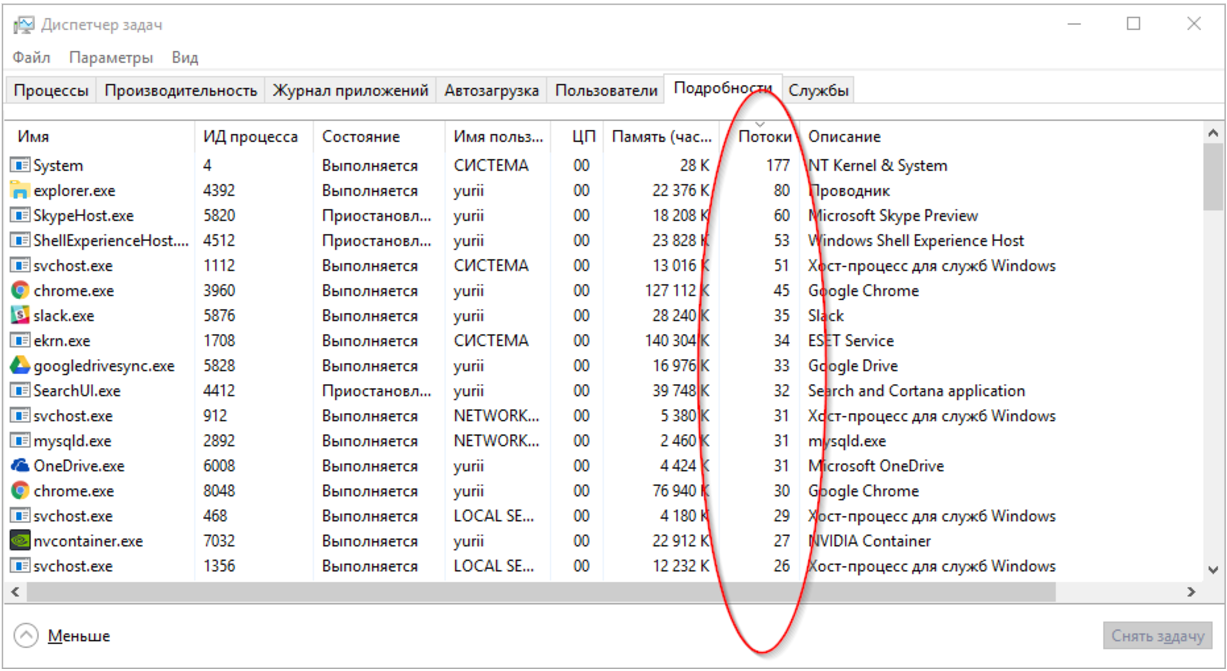
\includegraphics[width=0.8\textwidth]{threadsEverywhere.png}
\end{center}

Как видим, у проводника аж 80 потоков в одном процессе, у Скайпа --- 60. Отчасти это можно объяснить тем, что большая часть этого кода была написана до того, как пулы потоков стали модными, отчасти тем, что это, скорее всего, как раз потоки слежения за чем-нибудь --- они запустились, заблокировались на операции ввода-вывода и заснули, ожидая, когда что-нибудь произойдёт. То есть в планировании они не участвуют и ядра не занимают, но оперативку всё-таки кушают.

\section{Многопоточное программирование в .NET}

Конкретно в .NET функции операционной системы и планировщика обёрнуты в удобные классы пространства имён System.Threading. Класс Thread --- это тот самый низкоуровневый поток, которому можно передать функцию и запустить, и он будет её исполнять, пока она не досчитается, а затем закончит работу. Про пулы потоков мы поговорим на одной из следующих пар, домашку надо будет делать именно с Thread-ом. Вот минимальный пример многопоточной программы:

\begin{minted}{csharp}
namespace MultiThreadingDemo;

using System;
using System.Threading;

var otherThread = new Thread(() => 
{
    while (true)
    {
        Console.WriteLine("Hello from other thread!");
    }
});
otherThread.Start();

while (true)
{
    Console.WriteLine("Hello from this thread!");
}
\end{minted}

Как видим, Thread-у передаётся лямбда, которая в бесконечном цикле печатает что-то на экран. Мы его запускаем вызовом \mintinline{csharp}|otherThread.Start();|, этот вызов тут же возвращает управление и добавляет планировщику готовый к работе поток. При этом в основном потоке мы тоже запускаем бесконечный цикл. Результаты запуска программы демонстрируют кванты времени и неторопливость переключения потоков (на самом деле, там всё хитро, консоль синхронизирует вывод, но это детали).

\subsection{Параллельная обработка данных}

Теперь давайте сделаем что-нибудь более похожее на то, зачем нужна многопоточность. Положим, у нас есть большой массив, и мы хотим посчитать сумму его элементов. К счастью, алгебра говорит нам, что сложение ассоциативно, так что мы можем поделить массив на кусочки и поскладывать их в несколько потоков, а затем сложить только результаты. Вот код (уже без всяких using-ов):

\begin{small}
    \begin{minted}{csharp}
namespace MultiThreadingDemo;

using System;
using System.Threading;

var array = new int[] { 1, 5, 2, 4, 7, 2, 4, 9, 3, 6, 5 };
var threads = new Thread[3];
var chunkSize = array.Length / threads.Length + 1;
var results = new int[threads.Length];

for (var i = 0; i < threads.Length; ++i) {
    var localI = i;
    threads[i] = new Thread(() => {
        for (var j = localI * chunkSize; j < (localI + 1) * chunkSize && j < array.Length; ++j)
            results[localI] += array[j];
    });
}

foreach (var thread in threads)
    thread.Start();
foreach (var thread in threads)
    thread.Join();

var result = 0;
foreach (var subResult in results)
    result += subResult;

Console.WriteLine($"Result = {result}");
    \end{minted}
\end{small}

Создаём три потока, создаём массив результатов, для каждого потока вычисляем его кусок (так, чтобы каждый поток делал примерно одинаковую работу), передаём каждому потоку лямбду, которая считает сумму его куска (chunk) и записывает результат в массив результатов, в ячейку, равную номеру потока. Если вы помните про то, как работают замыкания в .NET, будет понятно, что за localI --- чтобы в каждую лямбду передавалась не ссылка на i, которая к моменту запуска потока будет содержать просто threads.Length, а текущее значение i, разное для каждого потока. Замыкания в .NET хранят значения <<по ссылке>>.

Подготовили потоки, запустили их, и --- новое по сравнению с предыдущим примером --- дождались завершения каждого методом \mintinline{csharp}|thread.Join();|. \mintinline{csharp}|thread.Join();| немедленно возвращает управление, если поток уже завершён, или блокирует вызвавший его поток, пока поток, у которого он был вызван, не завершится. Если поток, который мы хотим сджойнить, не завершится никогда, то и \mintinline{csharp}|thread.Join();| управление не вернёт, вызывающий тоже повиснет.

Ну и дальше в основном потоке без изысков сложили результаты и вывели то, что получилось, на экран.

\section{Проблемы синхронизации}

Выше приведена программа, суммирующая элементы массива, но она что-то какая-то сложная: там зачем-то заводится массив результатов и каждый поток пишет в свою ячейку, а затем ещё надо сложить числа в массиве результатов. Очевидно, можно проще, если суммировать в каждом потоке сразу в result:

\begin{small}
    \begin{minted}{csharp}
namespace MultiThreadingDemo;

using System;
using System.Threading;

var array = new int[] { 1, 5, 2, 4, 7, 2, 4, 9, 3, 6, 5 };
var threads = new Thread[3];
var chunkSize = array.Length / threads.Length + 1;
var result = 0;

for (var i = 0; i < threads.Length; ++i) {
    var localI = i;
    threads[i] = new Thread(() => {
        for (var j = localI * chunkSize; j < (localI + 1) * chunkSize && j < array.Length; ++j)
            result += array[j];
    });
}

foreach (var thread in threads)
    thread.Start();
foreach (var thread in threads)
    thread.Join();

Console.WriteLine($"Result = {result}");
    \end{minted}
\end{small}

Программа короче и менее заумная. Запускаем, проверяем, всё правильно работает (по крайней мере, у меня. Спойлер --- это дело случая, может и неправильный ответ выдать). Давайте попробуем, не меняя программу, увеличить размер задачи: сложить массив из тысячи единиц:

\begin{small}
    \begin{minted}{csharp}
namespace MultiThreadingDemo;

using System;
using System.Threading;

var array = new int[1000];
for (var i = 0; i < array.Length; ++i)
    array[i] = 1;

var threads = new Thread[8];
var chunkSize = array.Length / threads.Length + 1;
var result = 0;

for (var i = 0; i < threads.Length; ++i) {
    var localI = i;
    threads[i] = new Thread(() => {
        for (var j = localI * chunkSize; j < (localI + 1) * chunkSize && j < array.Length; ++j)
            result += array[j];
    });
}

foreach (var thread in threads)
    thread.Start();
foreach (var thread in threads)
    thread.Join();

Console.WriteLine($"Result = {result}");
    \end{minted}
\end{small}

Запускаем, проверяем, получаем тысячу. Всё ок. Запускаем ещё раз. Снова тысяча. Ещё раз. 980! Почему?

Дело в том, что размер задачи стал достаточно большим, чтобы она не считалась за один квант времени, так что в игру вступает планировщик. Планировщик, как вы помните, может прервать программу в любой момент, между любыми двумя инструкциями. Казалось бы, тут это не страшно, но вспомним, что C\# --- это высокоуровневый язык, который транслируется в байт-код .NET-машины, который, в свою очередь, JIT-компилируется в машинный код. Инструкции машинного кода, как правило, атомарны, в том смысле, что они либо исполняются целиком, либо не исполняются вовсе, и прерваны посередине быть не могут. А вот с нашей программой проблема становится очевидна уже на уровне байт-кода.

Строка \mintinline{csharp}|result += array[j];| транслируется в следующий набор инструкций .NET-машины:

\begin{footnotesize}
    \begin{minted}{text}
IL_0016: ldarg.0      // this
IL_0017: ldfld        class Program/'<>c__DisplayClass0_0' Program/'<>c__DisplayClass0_1'::'CS$<>8__locals1'
IL_001c: ldarg.0      // this
IL_001d: ldfld        class Program/'<>c__DisplayClass0_0' Program/'<>c__DisplayClass0_1'::'CS$<>8__locals1'
IL_0022: ldfld        int32 Program/'<>c__DisplayClass0_0'::result
IL_0027: ldarg.0      // this
IL_0028: ldfld        class Program/'<>c__DisplayClass0_0' Program/'<>c__DisplayClass0_1'::'CS$<>8__locals1'
IL_002d: ldfld        int32[] Program/'<>c__DisplayClass0_0'::'array'
IL_0032: ldloc.0      // j
IL_0033: ldelem.i4    
IL_0034: add          
IL_0035: stfld        int32 Program/'<>c__DisplayClass0_0'::result
    \end{minted}
\end{footnotesize}

Выглядит страшно, но суть в том, что сначала грузятся аргументы (и делается некая магия, определяющая, где в памяти лежит array[i], но она тут не имеет значения), затем выполняется сложение, затем сохраняется результат. Если \textbf{между} загрузкой аргументов и операцией записи результата в память произойдёт переключение потоков и управление получит другой поток, пытающийся выполнить ту же операцию, он считает \textbf{старое} значение result, запишет результат сложения, после чего снова произойдёт переключение потоков и наш первый поток запишет свой, уже посчитанный, но \textbf{старый} результат, тем самым перетерев результат соседнего потока. Поэтому ответ и получается меньше 1000 --- обычно потокам везёт, но иногда они портят результаты друг друга. А если ещё вспомнить, что современные процессоры многоядерные, потоки могут физически работать одновременно и физически одновременно выполнять доступ к памяти (к самой оперативке вряд ли, шина памяти не даст, но у ядер есть кеш...).

Итак, между \textbf{любыми двумя} инструкциями в машинном коде поток может быть прерван, и пока он не работает, в памяти может происходить масса интересных вещей. Даже \mintinline{csharp}|i++| в несколько потоков делать нельзя, если i --- разделяемая между потоками переменная, потому что внутри чтение, инкремент и запись делаются раздельно. Это, пожалуй, самое важное, что надо понимать о многопоточном программировании, всё остальное строится вокруг сего факта.

\subsection{Race condition}

Наблюдаемый в примере выше эффект обобщается до первой основной проблемы многопоточных программ --- race condition, или <<гонка>> в русскоязычной литературе. Формально, ситуация гонки --- это когда результат работы программы зависит от того, когда планировщик решил прервать поток и кому передать управление следующим. Ситуация гонки всегда означает ошибку и чаще всего возникает, когда потоки имеют разделяемые переменные, с которыми пытаются выполнять операции, не синхронизируясь. При этом читать из разделяемой переменной можно сколько угодно из скольки угодно потоков, а вот писать надо очень осторожно. Даже при одном <<писателе>> гонка может возникнуть из-за того, что <<читатели>> могут прочитать старое или новое значение переменной, в зависимости от того, как Бог кинул кости.

Вот простой пример:

\begin{center}
    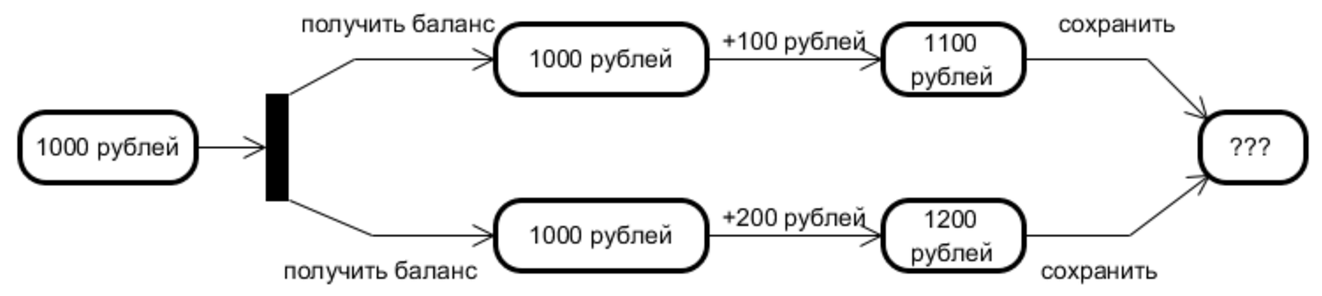
\includegraphics[width=0.8\textwidth]{raceCondition.png}
\end{center}

Хотим мы одновременно занести на счёт 100 рублей и 200 рублей. Ожидаем 1300 рублей, но в зависимости от того, как будут упорядочены инструкции первого и второго потока, мы можем получить, либо 1100, либо 1200, либо таки 1300 рублей. Как вы понимаете, в банковских системах гонки очень нежелательны.

\subsection{Deadlock}

Ещё один, более известный в теоретической литературе, хоть и немного более редкий на практике, пример проблем многопоточных программ --- это взаимоблокировка (Deadlock). Блокировка возникает тогда, когда:
\begin{enumerate}
    \item имеется разделяемый ресурс (например, файл), к которому потоки хотят получить доступ, но пользоваться им может только один поток, и пока он им пользуется, другие не могут его получить;
    \item таких ресурсов несколько и поток, захватив один, хочет получить доступ к другим (или другому), которые в этот момент захвачены другими потоками;
    \item нельзя отнять захваченный ресурс у потока;
    \item потоки ждут друг друга <<по кругу>> --- один ждёт ресурс, захваченный вторым, второй --- третьим, третий --- ..., N-й --- первым, и так как никто не может продолжить свою работу и отдать захваченный им ресурс, вся работа стоит, вечно.
\end{enumerate}

Рекомендую посмотреть визуализации в английской википедии\footnote{Deadlock, URL: \url{https://en.wikipedia.org/wiki/Deadlock}, дата обращения: 31.08.2020)} или на картинке: 

\begin{center}
    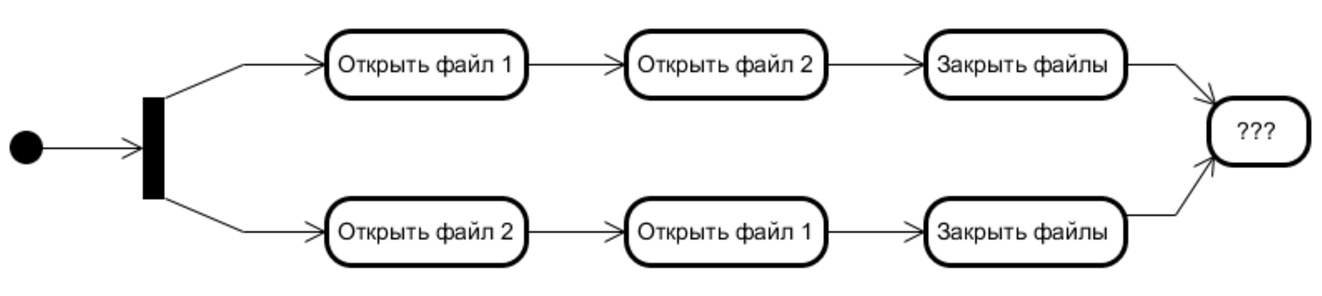
\includegraphics[width=0.8\textwidth]{deadlock.png}
\end{center}

Если всё сложится неудачно, верхний поток будет ждать, пока нижний освободит файл 2, а нижний будет ждать, пока верхний освободит файл 1, и они никогда не закончат работу.

Плохая новость в том, что блокировки бывают не только между потоками, но и между процессами, чего практически не бывает в случае с гонками. Хорошая новость в том, что блокировка возможна только в случае, если выполнены \textbf{все} условия, перечисленные выше. Чаще всего условие 1 есть суровая правда жизни, условие 2 есть часть бизнес-требований, условие 3 --- ограничение операционной системы (например, в Windows открытие файла блокирует вызвавший его поток, пока файл не освободят), а вот условие 4 зависит от программиста, поэтому взаимные блокировки легко избегаются, если перенумеровать разделяемые ресурсы и выдавать блокировки строго в порядке возрастания номеров. Тем не менее, блокировки можно легко добиться и без файлов --- попробуйте сделать Join() от текущего потока, например. Чтобы выполнить Join(), он должен завершиться, но чтобы завершиться, он должен подождать, пока Join() вернёт управление. На следующей неделе будет про примитивы синхронизации, они позволят ещё тысячей креативных способов оказаться в подобной ситуации.

\subsection{Чего ещё стоит опасаться}

Но и это ещё не все ужасы многопоточного программирования. Вот ещё пара интересных особенностей аппаратного обеспечения, про которые должен знать каждый программист:

\begin{itemize}
    \item Процессор может переставлять местами инструкции. Это не значит, что он может взять и испортить вашу программу --- результат исполнения гарантируется таким же, как и до перестановки. Но промежуточные результаты вычислений и промежуточные записи в память могут быть не такими, каких вы ожидаете. Делает это процессор не со зла, а для оптимизации исполнения на конвейере --- долгие инструкции, например, чтение из памяти, могут быть отложены на чуть попозже в надежде, что значение окажется в кеше. Другие ядра могут видеть неконсистентные состояния посреди счёта.
    \item У процессора есть кеш. Более того, у каждого ядра процессора есть два уровня кеша, конкретно этого ядра (L1 и L2), и общий для всех ядер и большой кеш L3. Так что когда вы пишете значение в память, то оно сначала оказывается в кеше L1, затем в кеше L2, затем в кеше L3, затем, через бесконечно долгие наносекунды, в памяти. Причём, пока значение ползёт в память, ядро продолжает работать, используя свой кеш как этакий образ памяти. Представьте, что два ядра исполняют одновременно два потока, каждый из которых выполняет инкремент одной переменной, просто x++. Сначала ядра читают значения из кеша, затем выполняют операцию инкремента (в арифметическом регистре), потом выгружают значение из регистра к себе в кеш L1, оттуда оно попадает в кеш L2 каждого ядра, и вот до того момента, пока значение не будет записано в L3, i --- это вообще две разные никак не связанные друг с другом переменные, со своими областями памяти в кешах ядер. При записи в L3 случится гонка. При этом в оперативке в переменной i может лежать вообще другое значение, про которое ядра даже не догадывались, потому что думали, что значение в их кешах актуально! На самом деле, не всё так ужасно, потому что кеши ядер аппаратно синхронизируются друг с другом, но и не так хорошо, потому что есть буферы чтения/записи между регистрами и кешом, они не синхронизируются (то есть все рассуждения про то, что ядро живёт в своей уютной реальности со своей уютной картиной мира, верно для буферов).
\end{itemize}

О том, как со всем этим жить, будет следующая лекция, оставайтесь с нами.

\end{document}
